\documentclass[a4paper, 12pt]{article}
\usepackage[T1]{fontenc}
\usepackage{lmodern}
\usepackage{color}
\usepackage{amsfonts}
\usepackage{epstopdf}
\usepackage{matlab}
\usepackage{booktabs}
%\documentclass{book}
\usepackage{blindtext}
\usepackage{hyperref}
\usepackage[brazil]{babel}
\usepackage{amssymb}
\usepackage[utf8]{inputenc}
\usepackage{amsmath}
\documentclass{article}
\usepackage{graphicx}
\usepackage{adjustbox}
\usepackage{float} % Para controle da posição das figuras
\usepackage{caption} % Para legendas customizadas

\usepackage{indentfirst}
\usepackage{graphicx}
\usepackage{listings}
\usepackage{tcolorbox}
\usepackage{upgreek}
\usepackage{multicol,lipsum}
\usepackage[a4paper,
top=3cm, left=3cm, bottom=3cm, right=3cm]{geometry}
\usepackage{setspace}
\usepackage{pdfpages}
\usepackage{multirow}
\usepackage{float}
\usepackage[dvipsnames]{xcolor}
\usepackage[table]{xcolor}
%\usepackage{pdflscape}
\usepackage[DIV=15]{typearea}
\usepackage[nottoc]{tocbibind}
\usepackage[sort,numbers]{natbib}
%\usepackage{cite}
\usepackage{matlab}
\newcommand{\uvec}[1]{\boldsymbol{\hat{\textbf{#1}}}}
\usepackage[utf8]{inputenc}
\usepackage[T1]{fontenc}
\usepackage{lmodern}
\usepackage{graphicx}
\usepackage{color}
\usepackage{hyperref}
\usepackage{amsmath}
\usepackage{amsfonts}
\usepackage{epstopdf}
\usepackage[table]{xcolor}
\usepackage{matlab}

\lstdefinestyle{python}{
  language=Python,
  basicstyle=\ttfamily,
  keywordstyle=\color{blue},
  stringstyle=\color{green},
  commentstyle=\color{gray},
  numbers=left,
  numberstyle=\tiny\color{gray},
  stepnumber=1,
  numbersep=5pt,
  backgroundcolor=\color{white},
  showspaces=false,
  showstringspaces=false,
  showtabs=false,
  frame=single,
  rulecolor=\color{black},
  tabsize=4,
  captionpos=b,
  breaklines=true,
  breakatwhitespace=false,
  title=\lstname,
  escapeinside={\%*}{*)},
  morekeywords={self},
  emph={MyClass,__init__},
  emphstyle=\color{red}
}


\documentclass[letterpaper]{article}
% bib pack %%%%%%%%%%%%%%%%%%%%%%%%%%%%%%%%%%%%%%%%%%%%%%%%%%%%%%%%%%%%%%%%%%%%%
\usepackage[utf8]{inputenc}
\usepackage{geometry}
    \geometry{left=3cm,right=2cm,top=2cm,bottom=2cm}
%
\usepackage[spanish]{babel}
%
\usepackage[fixlanguage]{babelbib}
    \bibliographystyle{babunsrt}
%
\usepackage{url}

\begin{document}
%\maketitle

\begin{titlepage}
	\begin{center}
		

\vspace{10pt}
%\begin{figure}[H][!ht]
%\centering
%
\includegraphics{puc-rio-logo.png}

%\end{figure}
\begin{figure}[!ht]
\centering

\includegraphics{images/puc-rio-logo.png}
\end{figure}
\huge{Controle Discreto}
        \vspace{70pt}
        
		\textbf{ENG1471}
		\textbf{\large{\\ }}
		
		\vspace{30pt}
		\textbf{\small{\\TRABALHO FINAL}}

		\vspace{75pt}
		
	\end{center}
	
	\begin{flushleft}
		\begin{tabbing}
		Aluno(a)\qquad\qquad\=\>Paloma Fernanda Loureiro Sette - 1621595\\

			Professor(a)\>Marco Antonio Meggiolaro\\
	\end{tabbing}
		  
	\end{flushleft}
	\begin{center}
		%\vspace{\fill}
		\vspace{215pt}
		Rio de Janeiro, 18 de Junho de 2024
	\end{center}
\end{titlepage}
%%%%%%%%%%%%%%%%%%%%%%%%%%%%%%%%%%%%%%%%%%%%%%%%%%%%%%%%%%%
\newpage
\tableofcontents
\thispagestyle{empty}

\newpage
\pagenumbering{arabic}

\newpage

%\newcommand{\listequationsname}{Lista de Equações}
%\newlistof{myequations}{equ}{\listequationsname}
%\newcommand{\myequations}[1]{%
%\addcontentsline{equ}{myequations}{\protect\numberline{\theequation}#1}\par}

%\listofmyequations
\newpage


\newpage

\listoffigures
\thispagestyle{empty}

\newpage
%%%%%%%%%%%%%%%%%%%%%%%%%%%%%%%%%%%%%%%%%%%%%%%%%%%%%%%%%
%%%%%%%%%%%%%%%%%%%%%%%%%%%%%%%%%%%%%%%%%%%%%%%%%%%

\newpage

\thispagestyle{empty}

\newpage

\section{Introdução}
Este relatório tem como objetivo descrever o desenvolvimento do trabalho final da disciplina de Controle Discreto. Este projeo consiste no desenvolvimento e na implementação de controladores discretos para um F/A-18E Super Hornet, garantindo especificações de desempenho e segurança durante uma missão crítica que envolve uma manobra de ataque e subsequente escape.\\
O controle de aeronaves modernas requer a implementação de estratégias avançadas que garantam não apenas a precisão na execução das manobras, mas também a segurança do piloto e da aeronave em condições adversas. O F/A-18E Super Hornet é uma aeronave de combate de alta performance. 

\subsection{Contexto e Objetivo}
O F/A-18E Super Hornet, em condições de combate, deve executar manobras complexas que incluem um mergulho até uma altitude muito baixa e, em seguida, uma rápida ascensão para uma altitude segura. Essas manobras precisam ser realizadas em um intervalo de tempo restrito e com limitações rigorosas de aceleração para preservar a integridade estrutural da aeronave e a segurança do piloto. O objetivo deste trabalho é projetar e simular controladores digitais que guiem a aeronave através dessa missão de forma eficiente, respeitando os limites impostos.

\subsection{Descrição do Sistema}
O sistema modelado considera a dinâmica longitudinal do F/A-18E, representada por um vetor de estado que inclui a velocidade longitudinal, a velocidade de ascensão, a taxa de arfagem, o ângulo de arfagem e a altitude. A ação de controle é aplicada através de desvios no ângulo do profundor e no empuxo, e o sistema está sujeito a perturbações externas, como vento.\\

O avião encontra-se horizontalmente em  velocidade de cruzeiro \textbf{uc = 375m/s} (Mach 1.1) a uma altitude inicial \textbf{h = h0 = 1000m}. Este F-18 precisa fazer uma manobra de ataque, mergulhando até uma altitude \textbf{h < hb = 20m}, e em seguida escapar ascendendo além de uma altitude segura \textbf{h > hf = 4000m}. Esta manobra completa precisa ser executada em um invervalo de tempo máximo \textbf{t } $\leq$ \textbf{tmax = 40s}.\\

O modelo Super Hornet do F-18 possui comprimento \textbf{L = 18.31m}, largura total \textbf{13.62m} (\textbf{8.4m} com as asas dobradas) e altura\textbf{ A = 4.88m}. Sua massa com combustível e todos os 
equipamentos necessários para essa missão é \textbf{M = 21538kg}, assumida constante durante a manobra. Esse modelo é atuado por dois turbofans General Electric F414-GE-400, cada um  capaz de prover até \textbf{98kN} de empuxo ao acionar o \textit{afterburner} (sem o \textit{afterburner} cairia para \textbf{58kN} cada), totalizando uma força conjunta \textbf{f} com um limite máximo \textbf{fmax = 196000N}
(\textbf{196kN}). A velocidade máxima teórica desse avião é \textbf{532m/s}, equivalente a Mach 1.6.\\

O avião foi projetado para operar de forma segura em até \textbf{7.6g}, onde \textbf{g = 9.81m/s$^2$} é a aceleração 
da gravidade local. No entanto, para essa missão serão admitidas acelerações máximas de até \textbf{10g}, acima das quais tanto a integridade do avião quanto do(a) piloto estariam em risco. A razão empuxo/peso do F-18 é definida como \textbf{fmax/(Mg)  $\cong$ 0.93}, e seu teto de serviço é de  cerca de \textbf{15000m}.

\begin{figure}[H]
\centering
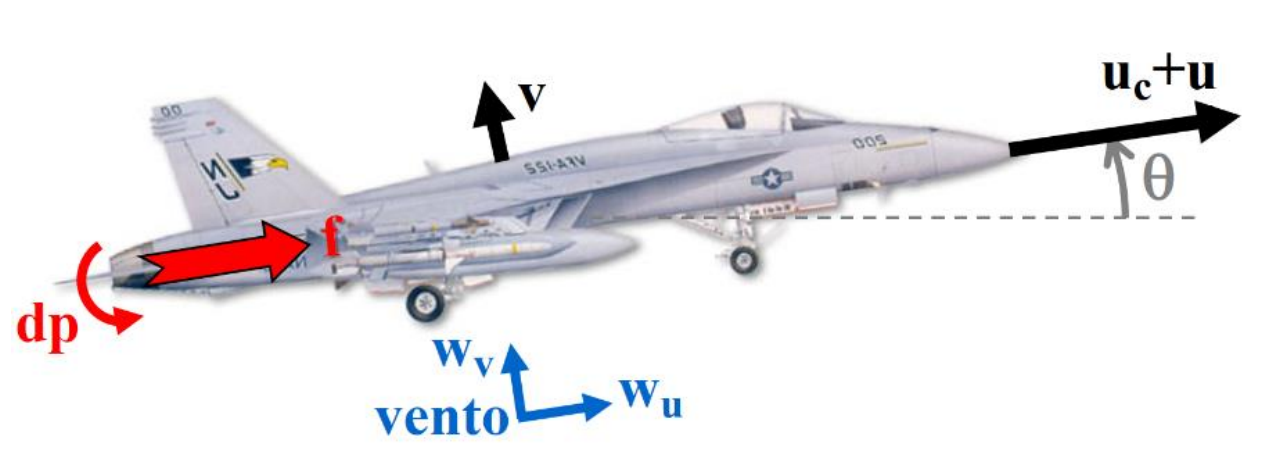
\includegraphics[scale = 0.30]{images/aviao.png}
\caption{F/A-18E Super Hornet}
\end{figure}


\newpage
\section{Considerações iniciais}
O vetor de estado \textbf{X} do F-18, que representa sua dinâmica longitudinal, é dado por
\begin{equation*}
    \mathbf{X} =  \begin{bmatrix}
       \mathbf{u} & \mathbf{v} & \boldsymbol{\dot \theta } & \boldsymbol{\theta} & \mathbf{h}
     \end{bmatrix}^T
\end{equation*}

Onde:

\begin{itemize}
    \item \textbf{(uc + u)} – velocidade longitudinal do F-18 (em relação a um referencial inercial no  solo, mas com direção definida ao longo da fuselagem) [m/s] – note que u seria o desvio da velocidade longitudinal em relação à de cruzeiro \textbf{uc = 375m/s}.
    \item \textbf{v} – velocidade de ascensão do F-18 (velocidade absoluta em relação ao solo, mas na  direção perpendicular à fuselagem) [m/s]
    \item $\boldsymbol{\dot \theta}$ – taxa de arfagem (\textit{pitch rate}, representando a velocidade angular do avião) [rad/s] 
    (por exemplo $\boldsymbol{\dot \theta}$ > 0 indicaria avião “empinando”), denominado tetap no Matlab;
    \item $\boldsymbol{\theta}$– ângulo de arfagem (pitch, ou inclinação) [rad] (por exemplo $\boldsymbol{\theta} > 0$ indicaria “nariz elevado”), denominado teta no Matlab;
    \item \textbf{h} – altitude em relação ao solo [m], medida na vertical.
\end{itemize}

Notemos que a condição inicial do problema é 
 $\mathbf{X_0} = \begin{bmatrix}
     \boldsymbol{0} & \boldsymbol{0} & \boldsymbol{0} & \boldsymbol{0} & \mathbf{h0} 
 \end{bmatrix}^T$
, que representa uma 
velocidade horizontal (e portanto \textbf{v = 0}, $\boldsymbol{\theta}= 0$ e $\boldsymbol{\theta}$ \textbf{= 0} e $\boldsymbol{\dot\theta}$ \textbf{= 0} ) igual a uc (e assim o desvio u = 0) em 
uma altitude inicial \textbf{h = h0 = 1000m}.\\

O vetor de atuação no avião é dado por \textbf{U = [dp de]$^T$}, onde:

\begin{itemize}
    \item \textbf{dp} – desvio no ângulo do profundor (\textit{taileron}, uma combinação de profundor e \textit{aileron} em sua cauda) em relação ao ângulo usado em cruzeiro [rad]; note os limites de operação \textbf{-0.5rad < dp < 0.5rad}, e que por exemplo um \textbf{dp > 0} abaixa o profundor  para provocar um “mergulho” do avião;
    \item \textbf{de }– empuxo (thrust) adimensionalizado, obtido dividindo a força conjunta\textbf{ f} dos  propulsores pela massa M do avião, isto é \textbf{de $\equiv$ f/M}, fazendo com que de sempre  fique no intervalo \textbf{0 < de $\leq$ fmax/M $\cong$ 9.1}. Note que esse limite superior \textbf{9.1} é igual ao  produto entre \textbf{g = 9.81m/s$^2$} e a razão empuxo/peso \textbf{0.93} do F-18 Super Hornet.
\end{itemize}

O avião está sujeito à perturbação do vento, dada pelo vetor \textbf{w = [$\mathbf{w_u}$ $\mathbf{w_v}$]$^T$}, onde:

\begin{itemize}
    \item  $\mathbf{w_u}$ – velocidade do vento em relação ao solo, na direção longitudinal do avião (ao  longo da fuselagem) [m/s];
    \item $\mathbf{w_v}$ -  velocidade do vento em relação ao solo, na direção perpendicular à fuselagem do  avião [m/s].
\end{itemize}

Assuma que o sistema abaixo represente o movimento desse avião. Ele foi linearizado para 
velocidades próximas à de cruzeiro uc e para altitudes h ao nível do mar. Note que o sistema 
também foi linearizado para $\boldsymbol{\theta}$ pequenos: por exemplo, a equação diferencial que rege a  altitude seria $\mathbf{\dot h = (u_c + u)sin(\boldsymbol{\theta}) + v cos(\boldsymbol{\theta})}$ , porém ao ser linearizada com $\mathbf{sin(\boldsymbol{\theta}) \cong \boldsymbol{\theta}}$, $\mathbf{cos(\boldsymbol{\theta}) \cong 1}$ e $\mathbf{u << u_c}$ ela resulta em $\mathbf{\dot h \cong u_c \boldsymbol{\theta} + v}$
, conforme representado abaixo. Por simplicidade, e 
para evitar a necessidade de implementar um simulador não-linear nesse problema, assume-se 
que o sistema linearizado abaixo seja válido para todas as altitudes\textbf{ h}, velocidades \textbf{($\mathbf{u_c}$ + u)} e
valores de $\boldsymbol{\theta}$ da manobra:

\begin{equation*}
    \mathbf{\dot X = FX + GU + G_Ww}
\end{equation*}

onde

\begin{figure}[H]
\centering
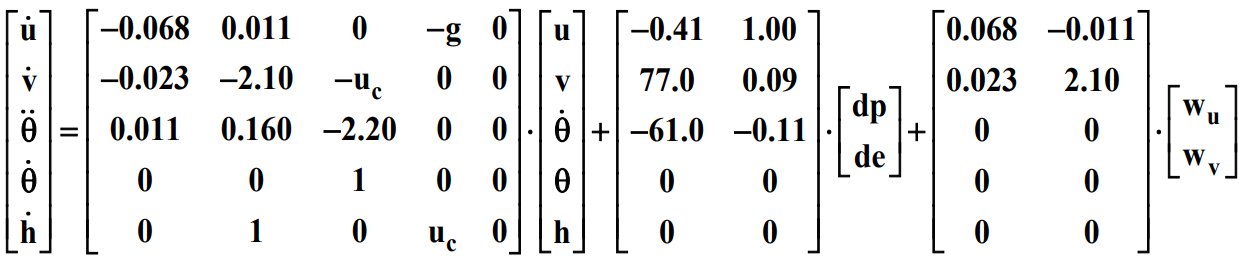
\includegraphics[scale = 0.37]{images/matrizes_op.png}
\end{figure}

Notemos que o sistema é altamente acoplado. Por exemplo, um aumento no empuxo adimensionalizado \textbf{de $\equiv$ f/M} provoca não só uma aceleração longitudinal $\mathbf{\dot u > 0}$
(com coeficiente \textbf{1.0}, como esperado pois 
$\mathbf{f = M\dot u}$ se todos os demais estados, atuações e perturbações forem nulos), mas também uma aceleração de ascensão $\mathbf{\dot v > 0}$ devido à maior sustentação gerada (coeficiente \textbf{0.09}), e até tende a fazer o avião “mergulhar” com a  aceleração angular $\mathbf{\ddot \theta < 0}$
(devido ao coeficiente negativo \textbf{-0.11}), o que pode ser explicado pelo fato de as turbinas se localizarem um pouco acima do centro de gravidade do avião, gerando um momento negativo.\\

Outro exemplo de acoplamento envolve abaixar o profundor devido a um valor \textbf{dp > 0}, que 
não apenas provoca a esperado tendência de “mergulho” do avião  $\mathbf{\ddot \theta < 0}$
(com coeficiente \textbf{-61.0}), como também gera uma aceleração vertical à fuselagem  $\mathbf{\dot v > 0}$ (coeficiente \textbf{77.0}) e 
uma frenagem longitudinal $\mathbf{\dot u < 0}$
(coeficiente \textbf{-0.41}) devido ao maior arrasto.\\

O controle do avião será feito de forma digital, mas assume-se que o controlador disponível
possui frequência de apenas \textbf{10Hz}, ou seja, \textbf{T = 0.1s} (período de controle \textbf{100ms}).\\

É fundamental definir uma trajetória de referência desejada $\mathbf{h_{desejada}}$ [m] para o controlador comparar com o valor medido/estimado de \textbf{h}, através de uma função temporal desde o 
instante inicial \textbf{t = 0} até o final \textbf{t = tfim = 50s} da simulação. É recomendável também (mas 
não necessário) especificar trajetórias de referência não nulas para as outras 4 variáveis de 
estado \textbf{u}, \textbf{v}, $\boldsymbol{\dot\theta}$
e $\boldsymbol{\theta}$, em função do tempo \textbf{t}, se isso ajudar no problema.\\

O controlador será considerado um sucesso se, e somente se:

\begin{itemize}
    \item a aceleração do F-18 jamais ultrapassar \textbf{10g} durante a manobra, para garantir a  integridade do avião e do(a) piloto;
    \item em algum instante da trajetória a altitude \textbf{h < hb = 20m }desejada for alcançada, e  sempre garantindo que \textbf{h > 0} para não haver colisão com o solo; e
    \item após \textbf{t = tmax = 40s} a altitude seja sempre \textbf{h > hf = 4000m}, para escapar com  segurança.
\end{itemize}




\newpage
\section{Estrutura do Trabalho}

O trabalho é dividido em duas partes principais:

\begin{itemize}
    \item \textbf{Parte 0:} Discretização do modelo contínuo do sistema usando a técnica de Zero-Order Hold (ZOH). São obtidas as matrizes equivalentes discretas que representam a dinâmica da aeronave em tempo discreto.
    \item \textbf{Parte 1:} Implementação de um controlador LQR para a manobra de mergulho e escape, assumindo condições ideais sem vento e com medições completas do estado. Nesta fase, determinamos os parâmetros ótimos do controlador e verificamos a resposta do sistema.
    \item \textbf{Parte 2:} Desenvolvimento de um controlador de emergência utilizando um filtro de Kalman, em cenários onde há presença de ventos e falha no sistema de navegação inercial. Esta parte lida com medições ruidosas e perturbações, ajustando a estratégia de controle para assegurar robustez sob condições adversas.
\end{itemize}




\section{Metodologia}
A abordagem adotada para o projeto e simulação dos controladores é baseada em técnicas clássicas de controle e filtragem, implementadas no ambiente MATLAB. As equações do modelo foram linearizadas e discretizadas para facilitar a simulação digital, e os controladores foram projetados com foco na estabilidade e no desempenho em tempo discreto. As simulações foram realizadas para verificar a aderência às especificações de desempenho e segurança.

\section{Resultados Esperados}
Espera-se que o controlador LQR implemente a manobra com sucesso, respeitando os limites de aceleração e atingindo as altitudes desejadas no tempo estipulado. Para o controlador de emergência, a expectativa é que o filtro de Kalman consiga fornecer estimativas robustas do estado, permitindo que a manobra seja realizada de forma segura mesmo em condições de perturbação e ruído.


\newpage
\section{Parte 0: Obtenção das Matrizes Discretas}

\subsection{1. Modelo Contínuo}

O sistema contínuo é dado pela equação:
\[
\dot{X}(t) = F X(t) + G U(t) + G_w w(t)
\]
com as matrizes fornecidas no problema:
\[
F = \begin{bmatrix}
-0.068 & 0.011 & 0 & -g & 0 \\
-0.023 & -2.10 & -u_c & 0 & 0 \\
0.011 & 0.160 & -2.20 & 0 & 0 \\
0 & 0 & 1 & 0 & 0 \\
0 & 1 & 0 & 0 & 0 
\end{bmatrix}
\]
\[
G = \begin{bmatrix}
-0.41 & 1.00 \\
77.0 & 0.09 \\
-61.0 & -0.11 \\
0 & 0 \\
0 & 0 
\end{bmatrix}
\]
\[
G_w = \begin{bmatrix}
0.068 & -0.011 \\
0.023 & 2.10 \\
0 & 0 \\
0 & 0 \\
0 & 0 
\end{bmatrix}
\]

\subsection*{2. Discretização usando ZOH}

A discretização ZOH envolve calcular as seguintes matrizes:
\[
\Phi = e^{FT}
\]
\[
\Gamma = \left( \int_0^T e^{F \tau} \, d\tau \right) G
\]
\[
\Gamma_w = \left( \int_0^T e^{F \tau} \, d\tau \right) G_w
\]
onde \( T \) é o período de amostragem. Para calcular isso, utilizamos o seguinte código MATLAB:

\begin{verbatim}
% Constantes fornecidas
g = 9.81;
u_c = 375;

% Matrizes fornecidas
F = [-0.068, 0.011, 0, -g, 0;
     -0.023, -2.10, -u_c, 0, 0;
     0.011, -0.160, -2.20, 0, 0;
     0, 0, 1, 0, 0;
     0, 1, 0, 0, 0];
 
G = [-0.41, 1.00;
     77.0, 0.09;
     -61.0, -0.11;
     0, 0;
     0, 0];
 
G_w = [0.068, -0.011;
       0.023, 2.10;
       0, 0;
       0, 0;
       0, 0];

T = 0.1; % Período de amostragem

% Criando sistema contínuo
sys_cont = ss(F, G, [], []);

% Discretizando com ZOH
sys_disc = c2d(sys_cont, T, 'zoh');

% Extraindo Phi e Gamma
Phi = sys_disc.A;
Gamma = sys_disc.B;

% Criando sistema contínuo para perturbações
sys_cont_w = ss(F, G_w, [], []);

% Discretizando com ZOH para perturbações
sys_disc_w = c2d(sys_cont_w, T, 'zoh');

% Extraindo Gamma_w
Gamma_w = sys_disc_w.B;

% Exibindo os resultados
disp('Phi = ');
disp(Phi);

disp('Gamma = ');
disp(Gamma);

disp('Gamma_w = ');
disp(Gamma_w);
\end{verbatim}

Os resultados das matrizes discretas são:

\begin{figure}[H]
\centering
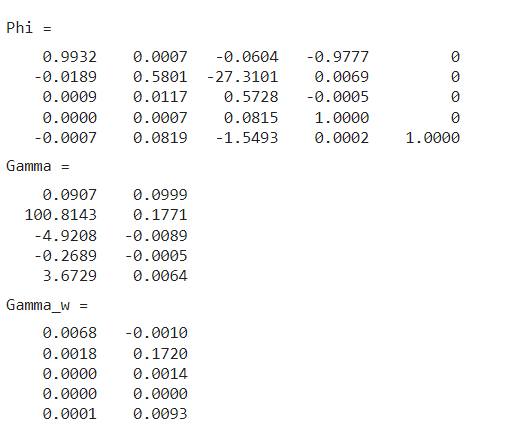
\includegraphics[scale = 0.90]{images/resultado_parte0.png}
\caption{Matrizes $\Phi$, $\Gamma$ e $\Gamma_w$ resultantes no MATLAB}
\end{figure}

As matrizes \( \Phi \), \( \Gamma \), e \( \Gamma_w \) foram calculadas com sucesso para a discretização do modelo contínuo do F/A-18E Super Hornet usando a técnica ZOH e os comandos \texttt{ss} e \texttt{c2d} para um período de amostragem de \( T = 0.1 \, \text{s} \). Essas matrizes serão utilizadas para simular o comportamento do sistema no domínio discreto nas próximas partes do trabalho.


\newpage
\section{Parte 1: Controle Longitudinal sem Perturbações}

Na Parte 1 do trabalho, implementamos um controlador Linear Quadratic Regulator (LQR) para o sistema de controle discreto do F/A-18E/F Super Hornet. O objetivo é conduzir a aeronave de uma altitude inicial \( h_0 = 1000 \, \text{m} \) para uma altitude final \( h_f = 4000 \, \text{m} \) no menor tempo possível, respeitando as restrições operacionais do sistema e garantindo a estabilidade durante a manobra.

\subsection{Modelo do Sistema}

O modelo do sistema foi linearizado e discretizado com Zero-Order Hold (ZOH). As matrizes do sistema contínuo são definidas como:

\[
F = \begin{bmatrix}
-0.068 & 0.011 & 0 & -g & 0 \\
-0.023 & -2.10 & -uc & 0 & 0 \\
0.011 & 0.160 & -2.20 & 0 & 0 \\
0 & 0 & 1 & 0 & 0 \\
0 & 1 & 0 & uc & 0
\end{bmatrix}
\]

\[
G = \begin{bmatrix}
-0.41 & 1.00 \\
77.0 & 0.09 \\
-61.0 & -0.11 \\
0 & 0 \\
0 & 0
\end{bmatrix}
\]

\[
G_w = \begin{bmatrix}
0.068 & -0.011 \\
0.023 & 2.10 \\
0 & 0 \\
0 & 0 \\
0 & 0
\end{bmatrix}
\]

onde \( g \) é a aceleração da gravidade e \( uc \) é a velocidade de cruzeiro.

\subsection{Configuração do Controlador LQR}

Para a implementação do controlador LQR, foram escolhidas as seguintes matrizes de peso \( Q_1 \) e \( Q_2 \):

\[
Q_1 = \text{diag}(1, 1, 8 \times 10^6, 2 \times 10^5, 1)
\]

\[
Q_2 = \text{diag}(10000, 93)
\]

Essas matrizes foram ajustadas para penalizar fortemente desvios nos estados relacionados à altitude \( h \) e ao ângulo de arfagem \( \theta \), garantindo que o controle seja suave e estável.

\subsection{ Implementação da Simulação}

A simulação foi conduzida com um período de controle \( T = 0.1 \, \text{s} \) durante 50 segundos. As variáveis de estado, \( X \), e as entradas de controle, \( U \), foram atualizadas conforme a seguinte lógica:

\begin{itemize}
    \item O estado inicial \( X_0 = [0, 0, 0, 0, h_0]^T \) foi definido com a altitude inicial \( h_0 \).
    \item Em cada iteração, calculamos a entrada de controle \( U \) utilizando a matriz de ganhos \( K \) do controlador LQR.
    \item Restrições foram aplicadas às entradas de controle:
    \[
    -0.5 \leq dp \leq 0.5 \quad \text{e} \quad 0 \leq de \leq 9.1
    \]
    \item A trajetória desejada \( X_d \) foi ajustada dinamicamente para garantir uma subida suave até a altitude final.
\end{itemize}

\subsection{ Resultados da Simulação}

A simulação demonstrou a eficácia do controlador LQR. O avião alcançou a altitude final \( h_f \) em aproximadamente 24,9 segundos, mantendo a estabilidade e respeitando as restrições operacionais. As principais métricas observadas foram:

\begin{itemize}
    \item Tempo da manobra: \( t_{\text{sucesso}} \approx 24.9 \, \text{s} \)
    \item Altitude mínima: \( h_{\text{min}} \approx 4.828 \, \text{m} \)
    \item Aceleração máxima: \( \frac{a}{g}_{\text{max}} \approx 9.899 \)
    \item Ângulo de arfagem máximo: \( \theta_{\text{max}} \approx 75.9089^\circ \)
    \item Máximo empuxo adimensional: \( de_{\text{max}} \approx 3.4907 \) (75 kN)
\end{itemize}

Os gráficos a seguir ilustram os resultados da simulação:

% Definição de uma nova página com a imagem
\newgeometry{left=0cm, right=0cm, top=0cm, bottom=0cm}
\begin{figure}[p]
    \centering
    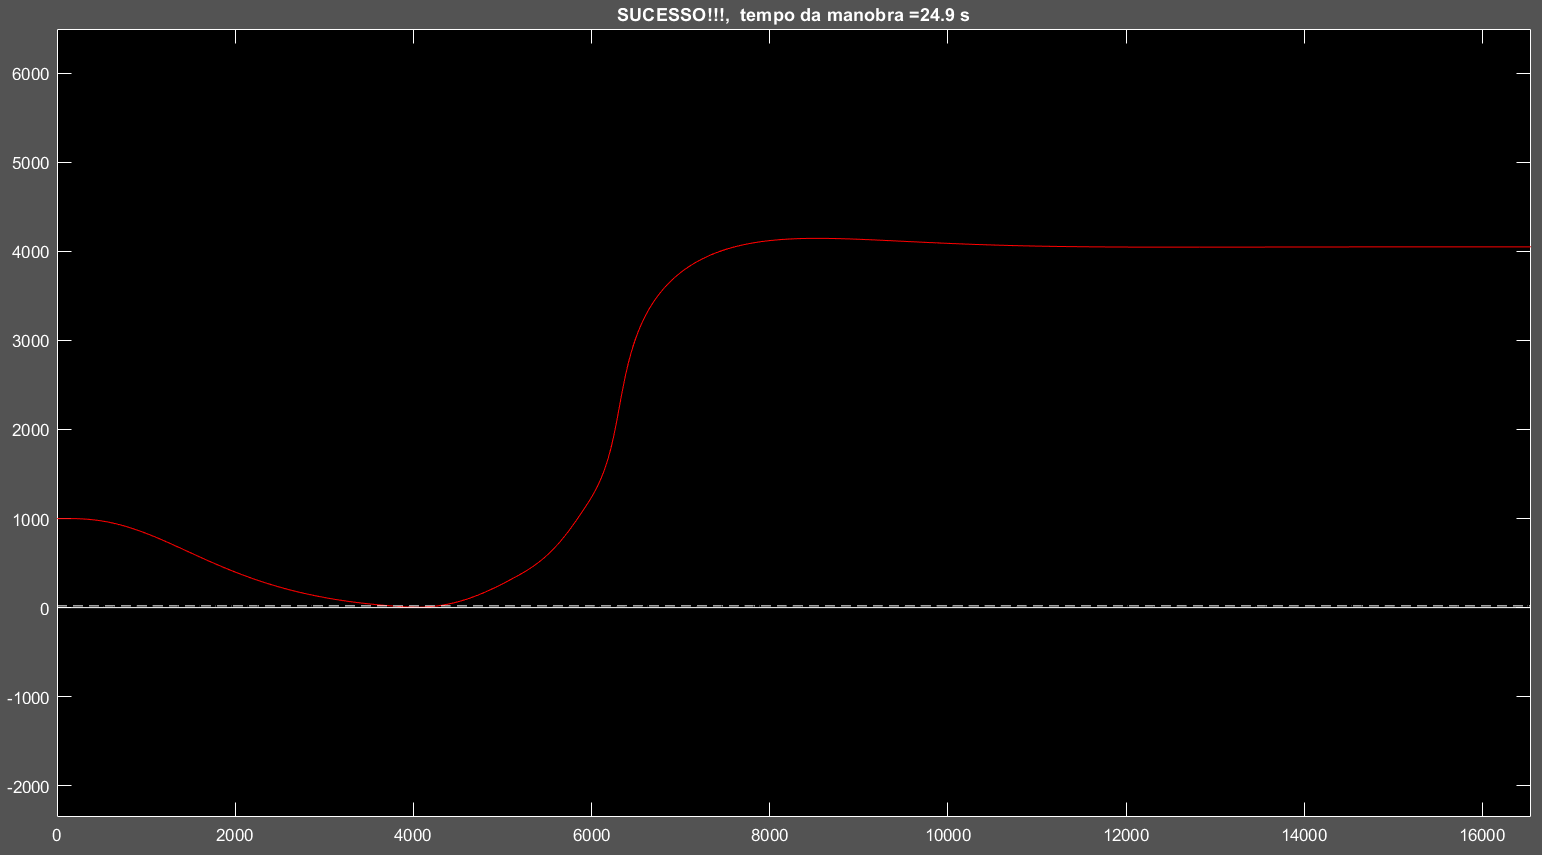
\includegraphics[width=\paperwidth, height=\paperheight, keepaspectratio]{images/sucesso.png}
    \caption{Altura em relação ao tempo, mostrando o sucesso da manobra.}
    \label{fig:imagem_pagina_inteira}
\end{figure}
\restoregeometry

% Definição de uma nova página com a imagem
\newgeometry{left=0cm, right=0cm, top=0cm, bottom=0cm}
\begin{figure}[p]
    \centering
    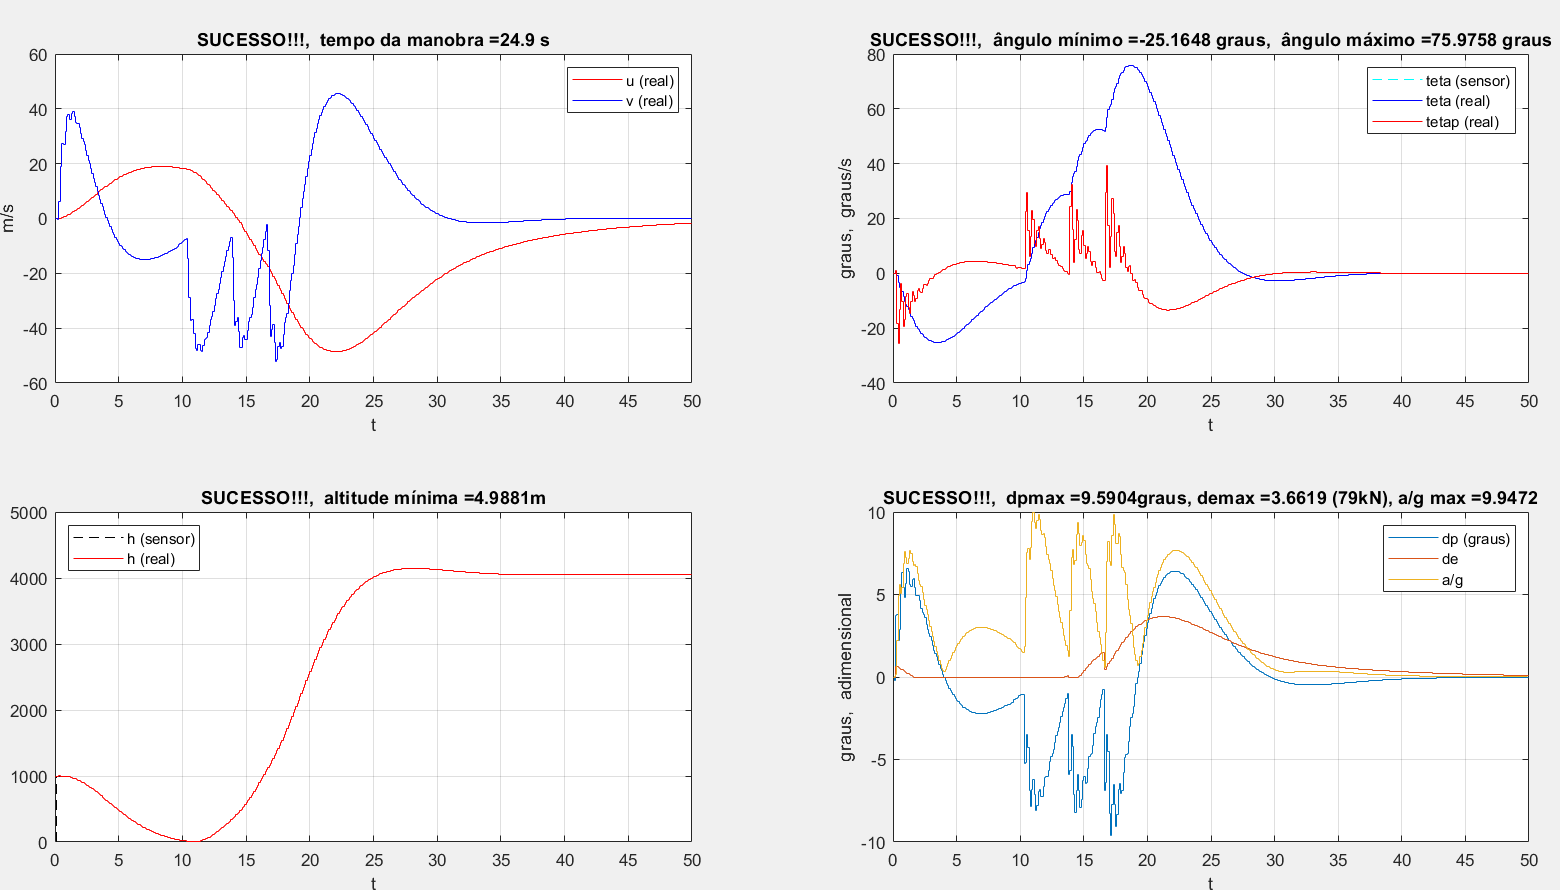
\includegraphics[width=\paperwidth, height=\paperheight, keepaspectratio]{images/resultado_parte1.png}
    \caption{Resultados da manobra: velocidade, ângulo de arfagem, altitude, e entradas de controle.}
\end{figure}
\restoregeometry

Implementamos com sucesso um controlador LQR para o sistema de controle discreto do F/A-18E/F Super Hornet. O controlador foi eficaz em conduzir o sistema ao estado desejado, respeitando as restrições e otimizando o tempo de manobra. A simulação mostrou que o controlador pode responder rapidamente às variações nos estados e manter a trajetória desejada de forma estável.

O código MATLAB detalhado utilizado para essa simulação encontra-se na seção de apêndice do relatório.




\newpage
\section{Parte 2: Controle Longitudinal com Perturbações e Ruídos}

Na Parte 2 do trabalho, o controle de emergência foi acionado devido à presença de turbulência significativa e falhas no sistema de navegação inercial. Utilizando apenas os sensores ruidosos de altímetro e inclinômetro, foi necessário implementar um filtro de Kalman para lidar com as condições adversas e tentar manter a estabilidade e controle da aeronave.

\subsection{Modelo do Sistema e Perturbações}

O modelo do sistema permaneceu o mesmo da Parte 1, com a inclusão de perturbações e ruídos. As perturbações do vento foram modeladas como velocidades aleatórias com desvio-padrão:

\[
w = \begin{bmatrix}
w_{u,\text{std}}^2 & 0 \\
0 & w_{v,\text{std}}^2
\end{bmatrix}
= \begin{bmatrix}
3^2 & 0 \\
0 & 2^2
\end{bmatrix}
\]

Os ruídos nos sensores foram representados pelas variâncias dos erros de medição:

\[
v_{\text{ruído}} = \begin{bmatrix}
h_{\text{std}}^2 \\
\theta_{\text{std}}^2
\end{bmatrix}
= \begin{bmatrix}
10^2 \\
0.0873^2
\end{bmatrix}
\]

\subsection{Implementação do Filtro de Kalman}

A implementação do filtro de Kalman envolveu as seguintes etapas:

\begin{enumerate}
    \item **Previsão**:
    \begin{itemize}
        \item Estimativa do estado futuro usando o modelo dinâmico.
        \item Atualização da incerteza do estado.
        \item Cálculo da estimativa da saída.
    \end{itemize}
    \item **Atualização**:
    \begin{itemize}
        \item Cálculo do erro da medição.
        \item Cálculo do ganho de Kalman.
        \item Atualização do estado e da covariância.
    \end{itemize}
\end{enumerate}

\subsection{Configuração do Controlador LQR}

As matrizes de peso \( Q_1 \) e \( Q_2 \) foram configuradas para a simulação com perturbações e ruídos como segue:

\[
Q_1 = \text{diag}(0.1, 1, 10^5, 5000, 0.2)
\]

\[
Q_2 = \text{diag}(5 \times 10^6, 20000)
\]

Estas matrizes foram escolhidas para priorizar a penalização dos estados que mais afetam a estabilidade e a segurança do voo, ao mesmo tempo que gerenciam os esforços de controle.

\subsection{Resultados da Simulação}

A simulação foi executada com um período de controle \( T = 0.1 \, \text{s} \) ao longo de 50 segundos. Observou-se que, em muitas execuções, a manobra foi bem-sucedida com um tempo de manobra de aproximadamente 40 segundos. No entanto, em algumas execuções, a simulação falhou devido a fatores como colisão no solo ou falha na altura final.

\begin{itemize}
    \item Tempo da manobra bem-sucedida: \( t_{\text{sucesso}} \approx 39.8 \, \text{s} \)
    \item Altitude mínima em casos de falha: variável
    \item Aceleração máxima em casos de falha: \( \frac{a}{g}_{\text{max}} > 10 \)
    \item Ângulo de arfagem máximo em casos de falha: variável
    \item Máximo empuxo adimensional em casos de falha: \( de_{\text{max}} \approx 9.1 \) (196 kN)
\end{itemize}



Os gráficos a seguir ilustram os resultados de uma execução típica da simulação:


% Definição de uma nova página com a imagem
\newgeometry{left=0cm, right=0cm, top=0cm, bottom=0cm}
\begin{figure}[p]
    \centering
    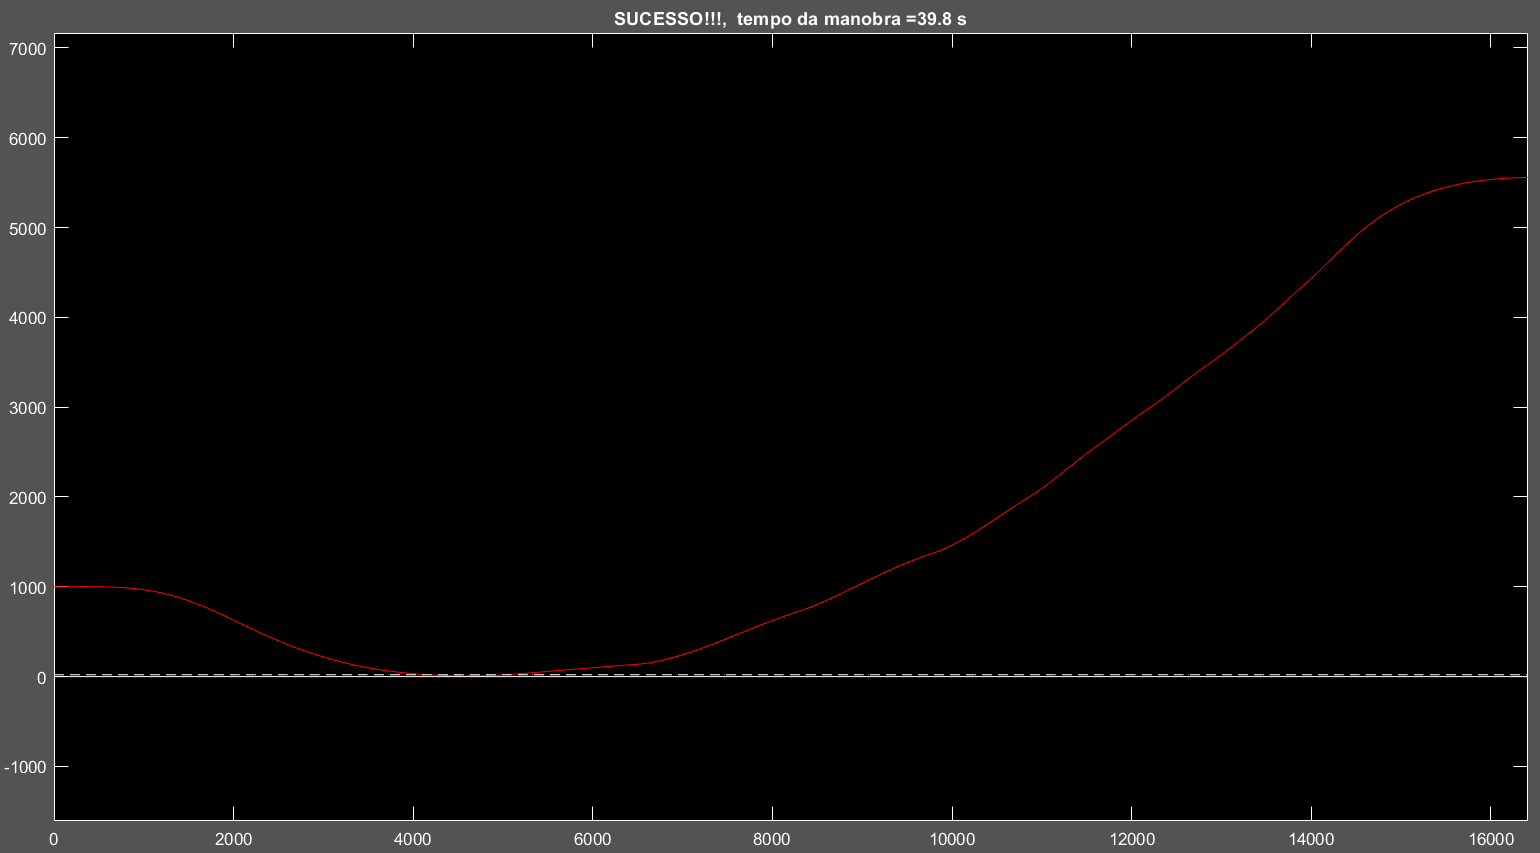
\includegraphics[width=\paperwidth, height=\paperheight, keepaspectratio]{images/sucesso_pt2.png}
    \caption{Gráfico resultando da manobra na Parte 2.}
    \label{fig:imagem_pagina_inteira_parte2}
\end{figure}
\restoregeometry

% Definição de uma nova página com a imagem
\newgeometry{left=0cm, right=0cm, top=0cm, bottom=0cm}
\begin{figure}[p]
    \centering
    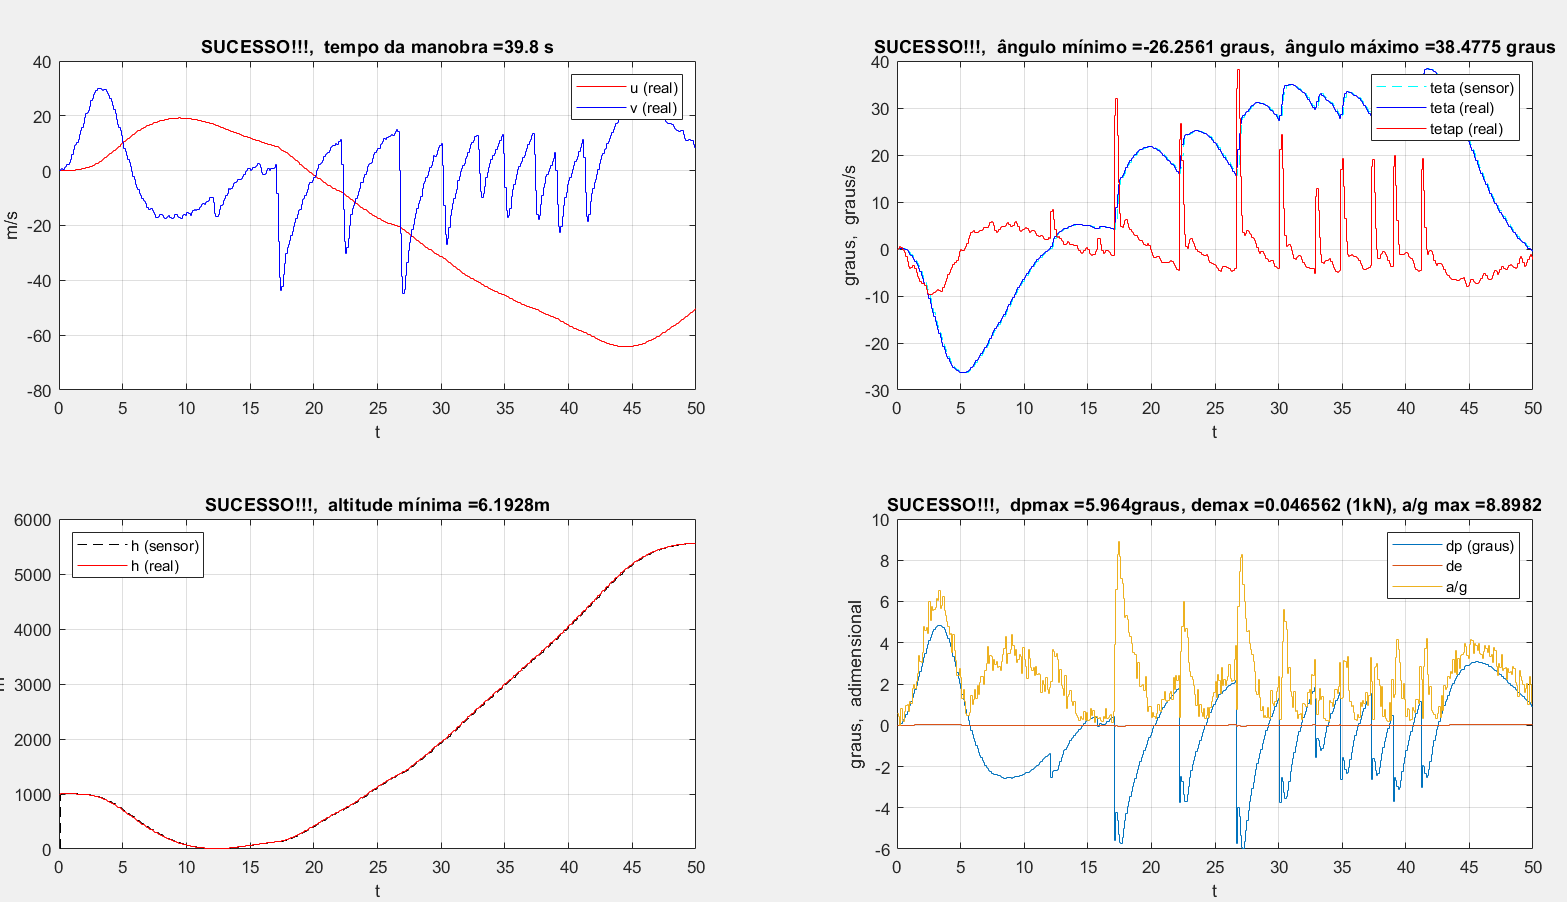
\includegraphics[width=\paperwidth, height=\paperheight, keepaspectratio]{images/resultado_parte2.png}
    \caption{Resultados da manobra na Parte 2.}
    \label{fig:imagem_pagina_inteira_parte2}
\end{figure}
\restoregeometry

\subsection{Justificativa para Casos de Falha}

Os casos de falha observados são atribuídos à natureza estocástica das perturbações e ruídos implementados no sistema. Devido à aleatoriedade desses fatores, as respostas do sistema variam a cada simulação, o que pode levar a situações em que o controle de emergência não consiga corrigir adequadamente a trajetória da aeronave a tempo, resultando em acelerações excessivas ou falha na altura final.

Esses resultados indicam que, embora o controlador LQR ajustado e o filtro de Kalman sejam eficazes em muitos cenários, ainda há necessidade de refinamentos para lidar consistentemente com todas as possíveis condições de perturbação e ruído.



\subsection{Complexidade do Filtro de Kalman no Contexto do Trabalho}

O filtro de Kalman aplicado neste trabalho desempenha um papel crucial na estabilização e controle do F/A-18E/F Super Hornet sob condições de ruído e perturbação. A complexidade de sua implementação reside na necessidade de estimar estados do sistema em tempo real, corrigindo previsões baseadas em medições ruidosas e atuando de maneira responsiva para minimizar os erros.

Implementar um filtro de Kalman eficiente para um sistema com alta variabilidade estocástica como o proposto apresenta vários desafios:

\begin{itemize}
    \item \textbf{**Estimativa de Estado com Ruído**}: O filtro de Kalman deve continuamente ajustar a estimativa do estado da aeronave com base em medições que são significativamente perturbadas por ruídos. Esse processo de atualização deve ser rápido e preciso para evitar desvios que possam comprometer o controle da aeronave.
    \item \textbf{**Sensibilidade às Condições Iniciais**}: Pequenas variações nas condições iniciais e na modelagem dos ruídos podem levar a grandes diferenças nos resultados. Isso exige uma calibragem meticulosa dos parâmetros do filtro de Kalman para garantir a robustez da solução.
    \item \textbf{**Integração com o Controlador LQR**}: O filtro de Kalman precisa trabalhar de forma coesa com o controlador LQR, fornecendo estados corrigidos que permitem ao LQR calcular ações de controle que mantenham a trajetória desejada. Esta integração deve lidar com a dinâmica rápida e complexa do sistema de controle.
    \item \textbf{**Adaptação a Condições Variáveis**}: Como o sistema está sujeito a perturbações aleatórias, o filtro de Kalman deve ser capaz de adaptar suas previsões e correções continuamente, o que aumenta a complexidade de sua implementação.
\end{itemize}

\subsection{Conclusões}

A implementação do filtro de Kalman combinada com o controlador LQR demonstrou ser uma abordagem robusta na maioria das simulações. No entanto, a presença de ruídos e perturbações estocásticas introduziu variabilidade nos resultados, com alguns casos de falha. Melhorias no modelo de controle e na sintonização dos parâmetros do filtro de Kalman podem ajudar a mitigar essas falhas e garantir a segurança e eficácia do controle em condições adversas.\\

Apesar das dificuldades, o uso do filtro de Kalman, junto com um controlador LQR bem ajustado, demonstrou ser uma técnica valiosa para lidar com as incertezas presentes no sistema e fornecer uma estimativa robusta dos estados da aeronave. No entanto, a complexidade envolvida reflete a necessidade de melhorias contínuas e testes extensivos para alcançar um desempenho consistente em todas as condições operacionais.






\newpage
\nocite{beer:ferdinand}
\nocite{janos:2005:algpseudocode}
\nocite{zandt:2010:fancyvrb}
\bibliography{referencias}

























% REFERENCIAS %%%%%%%%%%%%%%%%%%%%%%%%%%%%%%%%%%%%%%%%%%%%%%%%%%%%%%%%%%%%%%



\end{document}